\documentclass[twoside]{book}

% Packages required by doxygen
\usepackage{calc}
\usepackage{doxygen}
\usepackage{graphicx}
\usepackage[utf8]{inputenc}
\usepackage{makeidx}
\usepackage{multicol}
\usepackage{multirow}
\usepackage{textcomp}
\usepackage[table]{xcolor}

% Font selection
\usepackage[T1]{fontenc}
\usepackage{mathptmx}
\usepackage[scaled=.90]{helvet}
\usepackage{courier}
\usepackage{amssymb}
\usepackage{sectsty}
\renewcommand{\familydefault}{\sfdefault}
\allsectionsfont{%
  \fontseries{bc}\selectfont%
  \color{darkgray}%
}
\renewcommand{\DoxyLabelFont}{%
  \fontseries{bc}\selectfont%
  \color{darkgray}%
}

% Page & text layout
\usepackage{geometry}
\geometry{%
  a4paper,%
  top=2.5cm,%
  bottom=2.5cm,%
  left=2.5cm,%
  right=2.5cm%
}
\tolerance=750
\hfuzz=15pt
\hbadness=750
\setlength{\emergencystretch}{15pt}
\setlength{\parindent}{0cm}
\setlength{\parskip}{0.2cm}
\makeatletter
\renewcommand{\paragraph}{%
  \@startsection{paragraph}{4}{0ex}{-1.0ex}{1.0ex}{%
    \normalfont\normalsize\bfseries\SS@parafont%
  }%
}
\renewcommand{\subparagraph}{%
  \@startsection{subparagraph}{5}{0ex}{-1.0ex}{1.0ex}{%
    \normalfont\normalsize\bfseries\SS@subparafont%
  }%
}
\makeatother

% Headers & footers
\usepackage{fancyhdr}
\pagestyle{fancyplain}
\fancyhead[LE]{\fancyplain{}{\bfseries\thepage}}
\fancyhead[CE]{\fancyplain{}{}}
\fancyhead[RE]{\fancyplain{}{\bfseries\leftmark}}
\fancyhead[LO]{\fancyplain{}{\bfseries\rightmark}}
\fancyhead[CO]{\fancyplain{}{}}
\fancyhead[RO]{\fancyplain{}{\bfseries\thepage}}
\fancyfoot[LE]{\fancyplain{}{}}
\fancyfoot[CE]{\fancyplain{}{}}
\fancyfoot[RE]{\fancyplain{}{\bfseries\scriptsize Generated on Tue Feb 16 2016 22\-:21\-:25 for My Project by Doxygen }}
\fancyfoot[LO]{\fancyplain{}{\bfseries\scriptsize Generated on Tue Feb 16 2016 22\-:21\-:25 for My Project by Doxygen }}
\fancyfoot[CO]{\fancyplain{}{}}
\fancyfoot[RO]{\fancyplain{}{}}
\renewcommand{\footrulewidth}{0.4pt}
\renewcommand{\chaptermark}[1]{%
  \markboth{#1}{}%
}
\renewcommand{\sectionmark}[1]{%
  \markright{\thesection\ #1}%
}

% Indices & bibliography
\usepackage{natbib}
\usepackage[titles]{tocloft}
\setcounter{tocdepth}{3}
\setcounter{secnumdepth}{5}
\makeindex

% Hyperlinks (required, but should be loaded last)
\usepackage{ifpdf}
\ifpdf
  \usepackage[pdftex,pagebackref=true]{hyperref}
\else
  \usepackage[ps2pdf,pagebackref=true]{hyperref}
\fi
\hypersetup{%
  colorlinks=true,%
  linkcolor=blue,%
  citecolor=blue,%
  unicode%
}

% Custom commands
\newcommand{\clearemptydoublepage}{%
  \newpage{\pagestyle{empty}\cleardoublepage}%
}


%===== C O N T E N T S =====

\begin{document}

% Titlepage & ToC
\hypersetup{pageanchor=false}
\pagenumbering{roman}
\begin{titlepage}
\vspace*{7cm}
\begin{center}%
{\Large My Project }\\
\vspace*{1cm}
{\large Generated by Doxygen 1.8.6}\\
\vspace*{0.5cm}
{\small Tue Feb 16 2016 22:21:25}\\
\end{center}
\end{titlepage}
\clearemptydoublepage
\tableofcontents
\clearemptydoublepage
\pagenumbering{arabic}
\hypersetup{pageanchor=true}

%--- Begin generated contents ---
\chapter{Hierarchical Index}
\section{Class Hierarchy}
This inheritance list is sorted roughly, but not completely, alphabetically\-:\begin{DoxyCompactList}
\item \contentsline{section}{Bank\-Console\-U\-I\-C\-P\-P}{\pageref{classBankConsoleUICPP}}{}
\item \contentsline{section}{Bank\-C\-P\-P}{\pageref{classBankCPP}}{}
\item \contentsline{section}{Cm\-To\-Inch\-Console\-U\-I\-C\-P\-P}{\pageref{classCmToInchConsoleUICPP}}{}
\item \contentsline{section}{Cm\-To\-Inch\-C\-P\-P}{\pageref{classCmToInchCPP}}{}
\item exception\begin{DoxyCompactList}
\item \contentsline{section}{More\-Than\-Hundred}{\pageref{classMoreThanHundred}}{}
\item \contentsline{section}{Under\-Null\-Exception\-Cm}{\pageref{classUnderNullExceptionCm}}{}
\item \contentsline{section}{Under\-Null\-Exception\-H}{\pageref{classUnderNullExceptionH}}{}
\item \contentsline{section}{Under\-Null\-Exception\-Summa}{\pageref{classUnderNullExceptionSumma}}{}
\item \contentsline{section}{Under\-Null\-Exception\-W}{\pageref{classUnderNullExceptionW}}{}
\end{DoxyCompactList}
\item \contentsline{section}{Home\-Console\-U\-I\-C\-P\-P}{\pageref{classHomeConsoleUICPP}}{}
\item \contentsline{section}{Lib\-C\-P\-P}{\pageref{classLibCPP}}{}
\item \contentsline{section}{Matrix\-Console\-U\-I\-C\-P\-P}{\pageref{classMatrixConsoleUICPP}}{}
\item \contentsline{section}{Matrix\-C\-P\-P}{\pageref{classMatrixCPP}}{}
\item \contentsline{section}{Node}{\pageref{classNode}}{}
\item Q\-Object\begin{DoxyCompactList}
\item \contentsline{section}{Test\-C\-P\-P\-Test}{\pageref{classTestCPPTest}}{}
\item \contentsline{section}{Test\-Test}{\pageref{classTestTest}}{}
\end{DoxyCompactList}
\item \contentsline{section}{Rectangle}{\pageref{classRectangle}}{}
\item \contentsline{section}{Set}{\pageref{classSet}}{}
\item \contentsline{section}{Size}{\pageref{structSize}}{}
\item \contentsline{section}{Strings\-Console\-U\-I\-C\-P\-P}{\pageref{classStringsConsoleUICPP}}{}
\item \contentsline{section}{Strings\-C\-P\-P}{\pageref{classStringsCPP}}{}
\end{DoxyCompactList}

\chapter{Class Index}
\section{Class List}
Here are the classes, structs, unions and interfaces with brief descriptions\-:\begin{DoxyCompactList}
\item\contentsline{section}{\hyperlink{classBankConsoleUICPP}{Bank\-Console\-U\-I\-C\-P\-P} }{\pageref{classBankConsoleUICPP}}{}
\item\contentsline{section}{\hyperlink{classBankCPP}{Bank\-C\-P\-P} }{\pageref{classBankCPP}}{}
\item\contentsline{section}{\hyperlink{classCmToInchConsoleUICPP}{Cm\-To\-Inch\-Console\-U\-I\-C\-P\-P} }{\pageref{classCmToInchConsoleUICPP}}{}
\item\contentsline{section}{\hyperlink{classCmToInchCPP}{Cm\-To\-Inch\-C\-P\-P} }{\pageref{classCmToInchCPP}}{}
\item\contentsline{section}{\hyperlink{classHomeConsoleUICPP}{Home\-Console\-U\-I\-C\-P\-P} }{\pageref{classHomeConsoleUICPP}}{}
\item\contentsline{section}{\hyperlink{classLibCPP}{Lib\-C\-P\-P} }{\pageref{classLibCPP}}{}
\item\contentsline{section}{\hyperlink{classMatrixConsoleUICPP}{Matrix\-Console\-U\-I\-C\-P\-P} }{\pageref{classMatrixConsoleUICPP}}{}
\item\contentsline{section}{\hyperlink{classMatrixCPP}{Matrix\-C\-P\-P} }{\pageref{classMatrixCPP}}{}
\item\contentsline{section}{\hyperlink{classMoreThanHundred}{More\-Than\-Hundred} }{\pageref{classMoreThanHundred}}{}
\item\contentsline{section}{\hyperlink{classNode}{Node} }{\pageref{classNode}}{}
\item\contentsline{section}{\hyperlink{classRectangle}{Rectangle} }{\pageref{classRectangle}}{}
\item\contentsline{section}{\hyperlink{classSet}{Set} }{\pageref{classSet}}{}
\item\contentsline{section}{\hyperlink{structSize}{Size} }{\pageref{structSize}}{}
\item\contentsline{section}{\hyperlink{classStringsConsoleUICPP}{Strings\-Console\-U\-I\-C\-P\-P} }{\pageref{classStringsConsoleUICPP}}{}
\item\contentsline{section}{\hyperlink{classStringsCPP}{Strings\-C\-P\-P} }{\pageref{classStringsCPP}}{}
\item\contentsline{section}{\hyperlink{classTestCPPTest}{Test\-C\-P\-P\-Test} }{\pageref{classTestCPPTest}}{}
\item\contentsline{section}{\hyperlink{classTestTest}{Test\-Test} }{\pageref{classTestTest}}{}
\item\contentsline{section}{\hyperlink{classUnderNullExceptionCm}{Under\-Null\-Exception\-Cm} }{\pageref{classUnderNullExceptionCm}}{}
\item\contentsline{section}{\hyperlink{classUnderNullExceptionH}{Under\-Null\-Exception\-H} }{\pageref{classUnderNullExceptionH}}{}
\item\contentsline{section}{\hyperlink{classUnderNullExceptionSumma}{Under\-Null\-Exception\-Summa} }{\pageref{classUnderNullExceptionSumma}}{}
\item\contentsline{section}{\hyperlink{classUnderNullExceptionW}{Under\-Null\-Exception\-W} }{\pageref{classUnderNullExceptionW}}{}
\end{DoxyCompactList}

\chapter{Class Documentation}
\hypertarget{classBankConsoleUICPP}{\section{Bank\-Console\-U\-I\-C\-P\-P Class Reference}
\label{classBankConsoleUICPP}\index{Bank\-Console\-U\-I\-C\-P\-P@{Bank\-Console\-U\-I\-C\-P\-P}}
}
\subsection*{Public Member Functions}
\begin{DoxyCompactItemize}
\item 
\hypertarget{classBankConsoleUICPP_a2aa27548dcdea2c93b21674439e3e23a}{void {\bfseries do\-Work} ()}\label{classBankConsoleUICPP_a2aa27548dcdea2c93b21674439e3e23a}

\end{DoxyCompactItemize}


The documentation for this class was generated from the following files\-:\begin{DoxyCompactItemize}
\item 
app\-C\-P\-P/bankconsoleuicpp.\-h\item 
app\-C\-P\-P/bankconsoleuicpp.\-cpp\end{DoxyCompactItemize}

\hypertarget{classBankCPP}{\section{Bank\-C\-P\-P Class Reference}
\label{classBankCPP}\index{Bank\-C\-P\-P@{Bank\-C\-P\-P}}
}
\subsection*{Static Public Member Functions}
\begin{DoxyCompactItemize}
\item 
\hypertarget{classBankCPP_a27ce8653b4fe637389cedf8a44dd7828}{static double {\bfseries compound\-Interest} (double, double)}\label{classBankCPP_a27ce8653b4fe637389cedf8a44dd7828}

\end{DoxyCompactItemize}


The documentation for this class was generated from the following files\-:\begin{DoxyCompactItemize}
\item 
lib\-C\-P\-P/bankcpp.\-h\item 
lib\-C\-P\-P/bankcpp.\-cpp\end{DoxyCompactItemize}

\hypertarget{classCmToInchConsoleUICPP}{\section{Cm\-To\-Inch\-Console\-U\-I\-C\-P\-P Class Reference}
\label{classCmToInchConsoleUICPP}\index{Cm\-To\-Inch\-Console\-U\-I\-C\-P\-P@{Cm\-To\-Inch\-Console\-U\-I\-C\-P\-P}}
}
\subsection*{Public Member Functions}
\begin{DoxyCompactItemize}
\item 
\hypertarget{classCmToInchConsoleUICPP_a751dbd50f09391ebad00398c67c73b31}{void {\bfseries do\-Work} ()}\label{classCmToInchConsoleUICPP_a751dbd50f09391ebad00398c67c73b31}

\end{DoxyCompactItemize}


The documentation for this class was generated from the following files\-:\begin{DoxyCompactItemize}
\item 
app\-C\-P\-P/cmtoinchconsoleuicpp.\-h\item 
app\-C\-P\-P/cmtoinchconsoleuicpp.\-cpp\end{DoxyCompactItemize}

\hypertarget{classCmToInchCPP}{\section{Cm\-To\-Inch\-C\-P\-P Class Reference}
\label{classCmToInchCPP}\index{Cm\-To\-Inch\-C\-P\-P@{Cm\-To\-Inch\-C\-P\-P}}
}
\subsection*{Static Public Member Functions}
\begin{DoxyCompactItemize}
\item 
\hypertarget{classCmToInchCPP_a137509f38ad44e68e457afb92155cc94}{static double {\bfseries cm\-\_\-to\-\_\-inch} (double)}\label{classCmToInchCPP_a137509f38ad44e68e457afb92155cc94}

\item 
\hypertarget{classCmToInchCPP_a953aacbf7e8c3a63012db518555135ec}{static double {\bfseries inch\-\_\-to\-\_\-cm} (double)}\label{classCmToInchCPP_a953aacbf7e8c3a63012db518555135ec}

\end{DoxyCompactItemize}


The documentation for this class was generated from the following files\-:\begin{DoxyCompactItemize}
\item 
lib\-C\-P\-P/cmtoinchcpp.\-h\item 
lib\-C\-P\-P/cmtoinchcpp.\-cpp\end{DoxyCompactItemize}

\hypertarget{classHomeConsoleUICPP}{\section{Home\-Console\-U\-I\-C\-P\-P Class Reference}
\label{classHomeConsoleUICPP}\index{Home\-Console\-U\-I\-C\-P\-P@{Home\-Console\-U\-I\-C\-P\-P}}
}
\subsection*{Public Member Functions}
\begin{DoxyCompactItemize}
\item 
\hypertarget{classHomeConsoleUICPP_a021880cafb412c494569b845dbf8962d}{void {\bfseries do\-Work} ()}\label{classHomeConsoleUICPP_a021880cafb412c494569b845dbf8962d}

\end{DoxyCompactItemize}


The documentation for this class was generated from the following files\-:\begin{DoxyCompactItemize}
\item 
app\-C\-P\-P/homeconsoleuicpp.\-h\item 
app\-C\-P\-P/homeconsoleuicpp.\-cpp\end{DoxyCompactItemize}

\hypertarget{classLibCPP}{\section{Lib\-C\-P\-P Class Reference}
\label{classLibCPP}\index{Lib\-C\-P\-P@{Lib\-C\-P\-P}}
}


The documentation for this class was generated from the following file\-:\begin{DoxyCompactItemize}
\item 
lib\-C\-P\-P/libcpp.\-h\end{DoxyCompactItemize}

\hypertarget{classMatrixConsoleUICPP}{\section{Matrix\-Console\-U\-I\-C\-P\-P Class Reference}
\label{classMatrixConsoleUICPP}\index{Matrix\-Console\-U\-I\-C\-P\-P@{Matrix\-Console\-U\-I\-C\-P\-P}}
}
\subsection*{Public Member Functions}
\begin{DoxyCompactItemize}
\item 
\hypertarget{classMatrixConsoleUICPP_ab0044d76dfbcf421fa10ade07ba85833}{void {\bfseries do\-Work} (char $\ast$, char $\ast$)}\label{classMatrixConsoleUICPP_ab0044d76dfbcf421fa10ade07ba85833}

\item 
\hypertarget{classMatrixConsoleUICPP_a5aed2ba4c596c1cf98e8cb839e36b938}{void {\bfseries print\-Matrix} (\hyperlink{classMatrixCPP}{Matrix\-C\-P\-P})}\label{classMatrixConsoleUICPP_a5aed2ba4c596c1cf98e8cb839e36b938}

\end{DoxyCompactItemize}


The documentation for this class was generated from the following files\-:\begin{DoxyCompactItemize}
\item 
app\-C\-P\-P/matrixconsoleuicpp.\-h\item 
app\-C\-P\-P/matrixconsoleuicpp.\-cpp\end{DoxyCompactItemize}

\hypertarget{classMatrixCPP}{\section{Matrix\-C\-P\-P Class Reference}
\label{classMatrixCPP}\index{Matrix\-C\-P\-P@{Matrix\-C\-P\-P}}
}
\subsection*{Public Member Functions}
\begin{DoxyCompactItemize}
\item 
\hypertarget{classMatrixCPP_a1cf5289e2db47d32331cd4ba9a47183e}{{\bfseries Matrix\-C\-P\-P} (int height, int width)}\label{classMatrixCPP_a1cf5289e2db47d32331cd4ba9a47183e}

\item 
\hypertarget{classMatrixCPP_a0b7ec5d9204172c038f4c33a2a181284}{int {\bfseries get\-Cell} (int y, int x)}\label{classMatrixCPP_a0b7ec5d9204172c038f4c33a2a181284}

\item 
\hypertarget{classMatrixCPP_a53cc93fd486bbf7b52d8956da6d7a544}{int {\bfseries get\-Height} ()}\label{classMatrixCPP_a53cc93fd486bbf7b52d8956da6d7a544}

\item 
\hypertarget{classMatrixCPP_a2687dd04c1799009e6b1a7f6597a55a7}{int {\bfseries get\-Width} ()}\label{classMatrixCPP_a2687dd04c1799009e6b1a7f6597a55a7}

\end{DoxyCompactItemize}
\subsection*{Friends}
\begin{DoxyCompactItemize}
\item 
\hypertarget{classMatrixCPP_a4b8aa19337adf1bab977dd08bc81e177}{ostream \& {\bfseries operator$<$$<$} (ostream \&os, \hyperlink{classMatrixCPP}{Matrix\-C\-P\-P} \&matrix)}\label{classMatrixCPP_a4b8aa19337adf1bab977dd08bc81e177}

\end{DoxyCompactItemize}


The documentation for this class was generated from the following files\-:\begin{DoxyCompactItemize}
\item 
lib\-C\-P\-P/matrixcpp.\-h\item 
lib\-C\-P\-P/matrixcpp.\-cpp\end{DoxyCompactItemize}

\hypertarget{classMoreThanHundred}{\section{More\-Than\-Hundred Class Reference}
\label{classMoreThanHundred}\index{More\-Than\-Hundred@{More\-Than\-Hundred}}
}
Inheritance diagram for More\-Than\-Hundred\-:\begin{figure}[H]
\begin{center}
\leavevmode
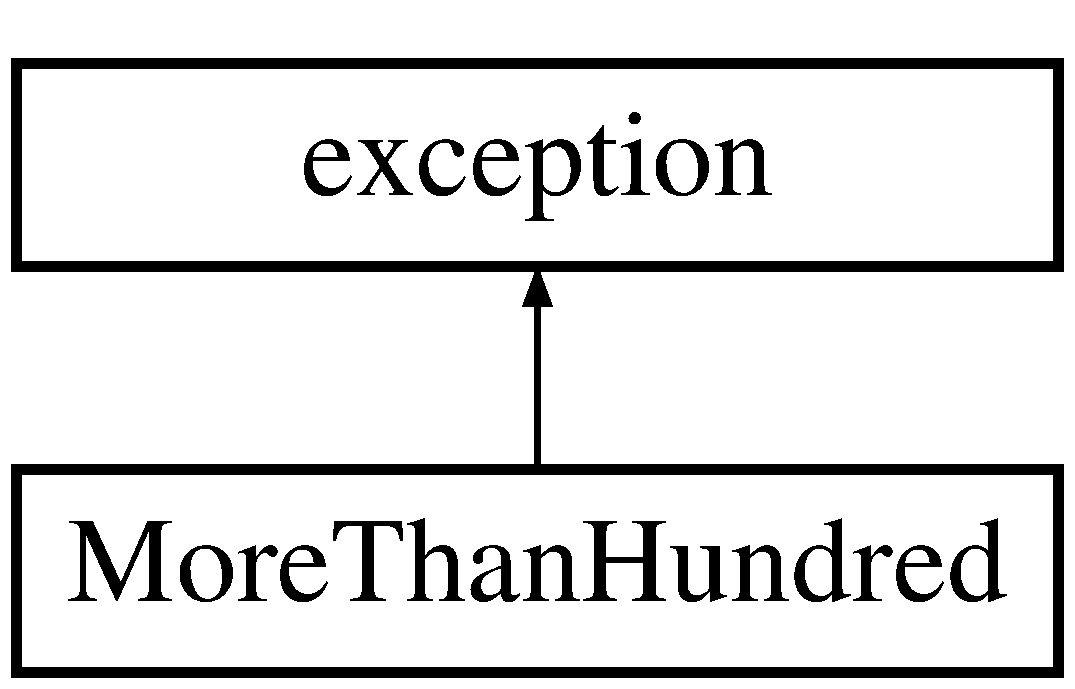
\includegraphics[height=2.000000cm]{classMoreThanHundred}
\end{center}
\end{figure}
\subsection*{Public Member Functions}
\begin{DoxyCompactItemize}
\item 
\hypertarget{classMoreThanHundred_a993286e53b7c3e39f6f4fddfc71a4be9}{{\bfseries More\-Than\-Hundred} (const int percent)}\label{classMoreThanHundred_a993286e53b7c3e39f6f4fddfc71a4be9}

\item 
\hypertarget{classMoreThanHundred_a89a337ca5c812c9f81f697ff25ff10c8}{int {\bfseries Get\-Percent} () const }\label{classMoreThanHundred_a89a337ca5c812c9f81f697ff25ff10c8}

\end{DoxyCompactItemize}


The documentation for this class was generated from the following file\-:\begin{DoxyCompactItemize}
\item 
lib\-C\-P\-P/exception.\-h\end{DoxyCompactItemize}

\hypertarget{classNode}{\section{Node Class Reference}
\label{classNode}\index{Node@{Node}}
}
\subsection*{Public Member Functions}
\begin{DoxyCompactItemize}
\item 
\hypertarget{classNode_aff71d952af8363f046a67a8b12194e46}{{\bfseries Node} (int)}\label{classNode_aff71d952af8363f046a67a8b12194e46}

\item 
\hypertarget{classNode_aff31c12e14a6f00952a46ff967db0c96}{{\bfseries Node} (int, \hyperlink{classNode}{Node} $\ast$)}\label{classNode_aff31c12e14a6f00952a46ff967db0c96}

\item 
\hypertarget{classNode_a2da744e4e704b0e2684e0d7476cf8c26}{void {\bfseries set\-Data} (int data)}\label{classNode_a2da744e4e704b0e2684e0d7476cf8c26}

\item 
\hypertarget{classNode_ae0062432733265c491000494625c3a04}{void {\bfseries set\-Next} (\hyperlink{classNode}{Node} $\ast$next)}\label{classNode_ae0062432733265c491000494625c3a04}

\item 
\hypertarget{classNode_aca98907146d5d0687f48bf8be9df9b7d}{int {\bfseries get\-Data} ()}\label{classNode_aca98907146d5d0687f48bf8be9df9b7d}

\item 
\hypertarget{classNode_ae36639ff267d63e058ce309fde5a9913}{\hyperlink{classNode}{Node} $\ast$ {\bfseries get\-Next} ()}\label{classNode_ae36639ff267d63e058ce309fde5a9913}

\end{DoxyCompactItemize}


The documentation for this class was generated from the following files\-:\begin{DoxyCompactItemize}
\item 
set/node.\-h\item 
set/node.\-cpp\end{DoxyCompactItemize}

\hypertarget{classRectangle}{\section{Rectangle Class Reference}
\label{classRectangle}\index{Rectangle@{Rectangle}}
}
\subsection*{Public Member Functions}
\begin{DoxyCompactItemize}
\item 
\hypertarget{classRectangle_a8c1bc640c993e1284e191b0c2c0e9acb}{{\bfseries Rectangle} (const double width, const double height)}\label{classRectangle_a8c1bc640c993e1284e191b0c2c0e9acb}

\item 
\hypertarget{classRectangle_ab750e4f0666df9c303ad649342bf3efd}{int {\bfseries get\-Width} ()}\label{classRectangle_ab750e4f0666df9c303ad649342bf3efd}

\item 
\hypertarget{classRectangle_a85fd455c8fda2674f857e04a116b8e62}{void {\bfseries set\-Width} (const double width)}\label{classRectangle_a85fd455c8fda2674f857e04a116b8e62}

\item 
\hypertarget{classRectangle_a9b6909485e6cc6e33717c6fba0d29761}{int {\bfseries get\-Height} ()}\label{classRectangle_a9b6909485e6cc6e33717c6fba0d29761}

\item 
\hypertarget{classRectangle_a8dc3f8324fbc25be80fe8888db717574}{void {\bfseries set\-Height} (const double height)}\label{classRectangle_a8dc3f8324fbc25be80fe8888db717574}

\item 
\hypertarget{classRectangle_a3c08182270dfee26126bafc80da5ca3d}{bool {\bfseries can\-Insert} (\hyperlink{classRectangle}{Rectangle}, \hyperlink{classRectangle}{Rectangle})}\label{classRectangle_a3c08182270dfee26126bafc80da5ca3d}

\end{DoxyCompactItemize}


The documentation for this class was generated from the following files\-:\begin{DoxyCompactItemize}
\item 
lib\-C\-P\-P/rectangle.\-h\item 
lib\-C\-P\-P/rectangle.\-cpp\end{DoxyCompactItemize}

\hypertarget{classSet}{\section{Set Class Reference}
\label{classSet}\index{Set@{Set}}
}
\subsection*{Public Member Functions}
\begin{DoxyCompactItemize}
\item 
\hypertarget{classSet_ade278ae4c854ce7d0f1f30cf8a7261c0}{{\bfseries Set} (const \hyperlink{classSet}{Set} \&source)}\label{classSet_ade278ae4c854ce7d0f1f30cf8a7261c0}

\item 
\hypertarget{classSet_a82601c80c4b9339e72260a812e956241}{void {\bfseries add} (int)}\label{classSet_a82601c80c4b9339e72260a812e956241}

\item 
\hypertarget{classSet_ac5ac16d671114a84654a68b14fea6d19}{void {\bfseries add} (\hyperlink{classSet}{Set})}\label{classSet_ac5ac16d671114a84654a68b14fea6d19}

\item 
\hypertarget{classSet_a08d9b0d8235e946c6afd5234aa536fb3}{bool {\bfseries contains} (int)}\label{classSet_a08d9b0d8235e946c6afd5234aa536fb3}

\item 
\hypertarget{classSet_affd89ff0f9ea60f4b3f15ed2b9b53f26}{bool {\bfseries contains} (\hyperlink{classSet}{Set})}\label{classSet_affd89ff0f9ea60f4b3f15ed2b9b53f26}

\item 
\hypertarget{classSet_acb80e4086c16baa5a0ab5d1e7fb8c2d7}{\hyperlink{classSet}{Set} {\bfseries copy} (\hyperlink{classSet}{Set})}\label{classSet_acb80e4086c16baa5a0ab5d1e7fb8c2d7}

\item 
\hypertarget{classSet_a33e855c52d34503a59b153827d0df774}{\hyperlink{classSet}{Set} {\bfseries intersect} (\hyperlink{classSet}{Set} s)}\label{classSet_a33e855c52d34503a59b153827d0df774}

\item 
\hypertarget{classSet_a4b34de1f00e7a96b7199ef0018324956}{int {\bfseries count} ()}\label{classSet_a4b34de1f00e7a96b7199ef0018324956}

\item 
\hypertarget{classSet_a46ae39a6de21c896881a25a26289c599}{bool {\bfseries is\-Empty} ()}\label{classSet_a46ae39a6de21c896881a25a26289c599}

\end{DoxyCompactItemize}


The documentation for this class was generated from the following files\-:\begin{DoxyCompactItemize}
\item 
set/set.\-h\item 
set/set.\-cpp\end{DoxyCompactItemize}

\hypertarget{structSize}{\section{Size Struct Reference}
\label{structSize}\index{Size@{Size}}
}
\subsection*{Public Attributes}
\begin{DoxyCompactItemize}
\item 
\hypertarget{structSize_a46feb84f0ac34e6b88eab63a0bf6601e}{double {\bfseries width}}\label{structSize_a46feb84f0ac34e6b88eab63a0bf6601e}

\item 
\hypertarget{structSize_a0222024b6e039f76ff8fce795dc0ec6c}{double {\bfseries height}}\label{structSize_a0222024b6e039f76ff8fce795dc0ec6c}

\end{DoxyCompactItemize}


The documentation for this struct was generated from the following file\-:\begin{DoxyCompactItemize}
\item 
lib/home.\-h\end{DoxyCompactItemize}

\hypertarget{classStringsConsoleUICPP}{\section{Strings\-Console\-U\-I\-C\-P\-P Class Reference}
\label{classStringsConsoleUICPP}\index{Strings\-Console\-U\-I\-C\-P\-P@{Strings\-Console\-U\-I\-C\-P\-P}}
}
\subsection*{Public Member Functions}
\begin{DoxyCompactItemize}
\item 
\hypertarget{classStringsConsoleUICPP_a6eb6ebbf3e7692efe4c9f9cd6ad63a6e}{void {\bfseries do\-Work} ()}\label{classStringsConsoleUICPP_a6eb6ebbf3e7692efe4c9f9cd6ad63a6e}

\end{DoxyCompactItemize}


The documentation for this class was generated from the following files\-:\begin{DoxyCompactItemize}
\item 
app\-C\-P\-P/stringsconsoleuicpp.\-h\item 
app\-C\-P\-P/stringsconsoleuicpp.\-cpp\end{DoxyCompactItemize}

\hypertarget{classStringsCPP}{\section{Strings\-C\-P\-P Class Reference}
\label{classStringsCPP}\index{Strings\-C\-P\-P@{Strings\-C\-P\-P}}
}
\subsection*{Static Public Member Functions}
\begin{DoxyCompactItemize}
\item 
\hypertarget{classStringsCPP_ae478b8a05e718fa0dca8d6c81b7477c2}{static void {\bfseries spread\-\_\-text} (string $\ast$text, int lines)}\label{classStringsCPP_ae478b8a05e718fa0dca8d6c81b7477c2}

\end{DoxyCompactItemize}


The documentation for this class was generated from the following files\-:\begin{DoxyCompactItemize}
\item 
lib\-C\-P\-P/stringscpp.\-h\item 
lib\-C\-P\-P/stringscpp.\-cpp\end{DoxyCompactItemize}

\hypertarget{classTestCPPTest}{\section{Test\-C\-P\-P\-Test Class Reference}
\label{classTestCPPTest}\index{Test\-C\-P\-P\-Test@{Test\-C\-P\-P\-Test}}
}
Inheritance diagram for Test\-C\-P\-P\-Test\-:\begin{figure}[H]
\begin{center}
\leavevmode
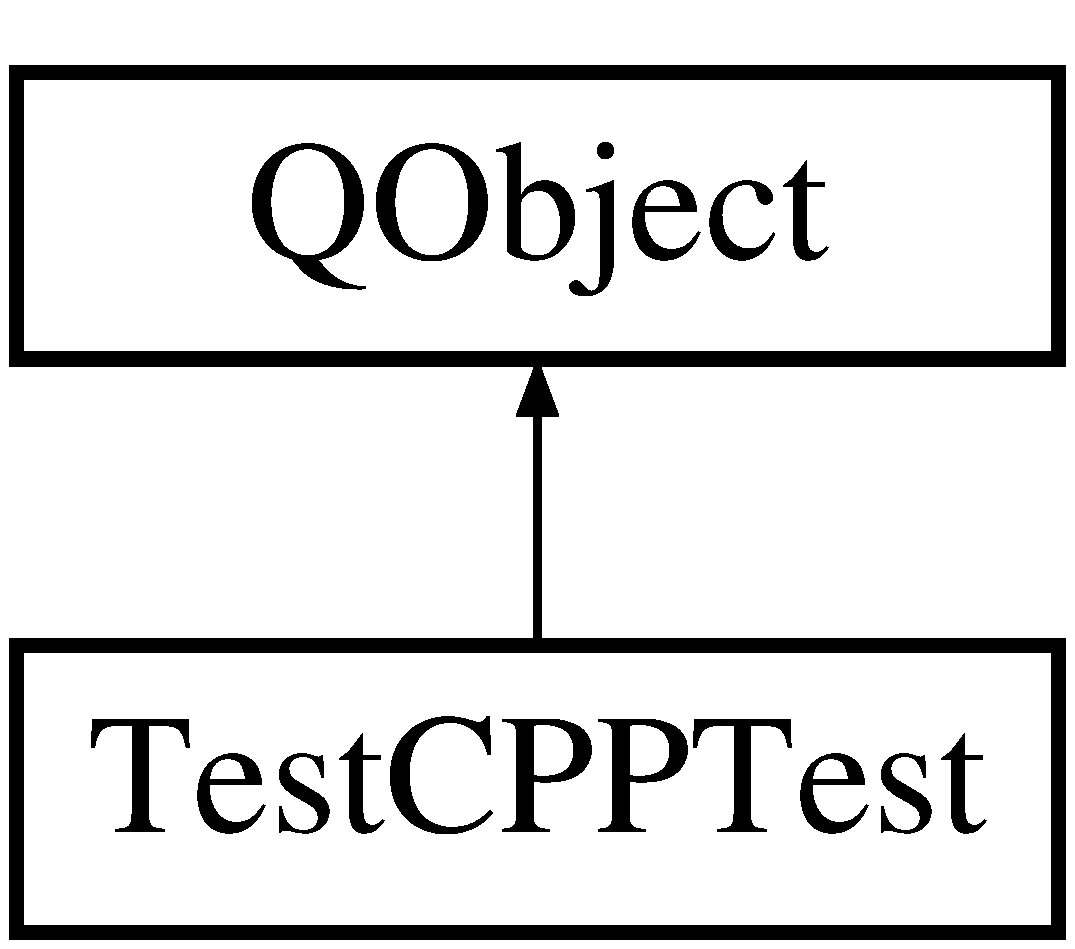
\includegraphics[height=2.000000cm]{classTestCPPTest}
\end{center}
\end{figure}


The documentation for this class was generated from the following file\-:\begin{DoxyCompactItemize}
\item 
test\-C\-P\-P/tst\-\_\-testcpptest.\-cpp\end{DoxyCompactItemize}

\hypertarget{classTestTest}{\section{Test\-Test Class Reference}
\label{classTestTest}\index{Test\-Test@{Test\-Test}}
}
Inheritance diagram for Test\-Test\-:\begin{figure}[H]
\begin{center}
\leavevmode
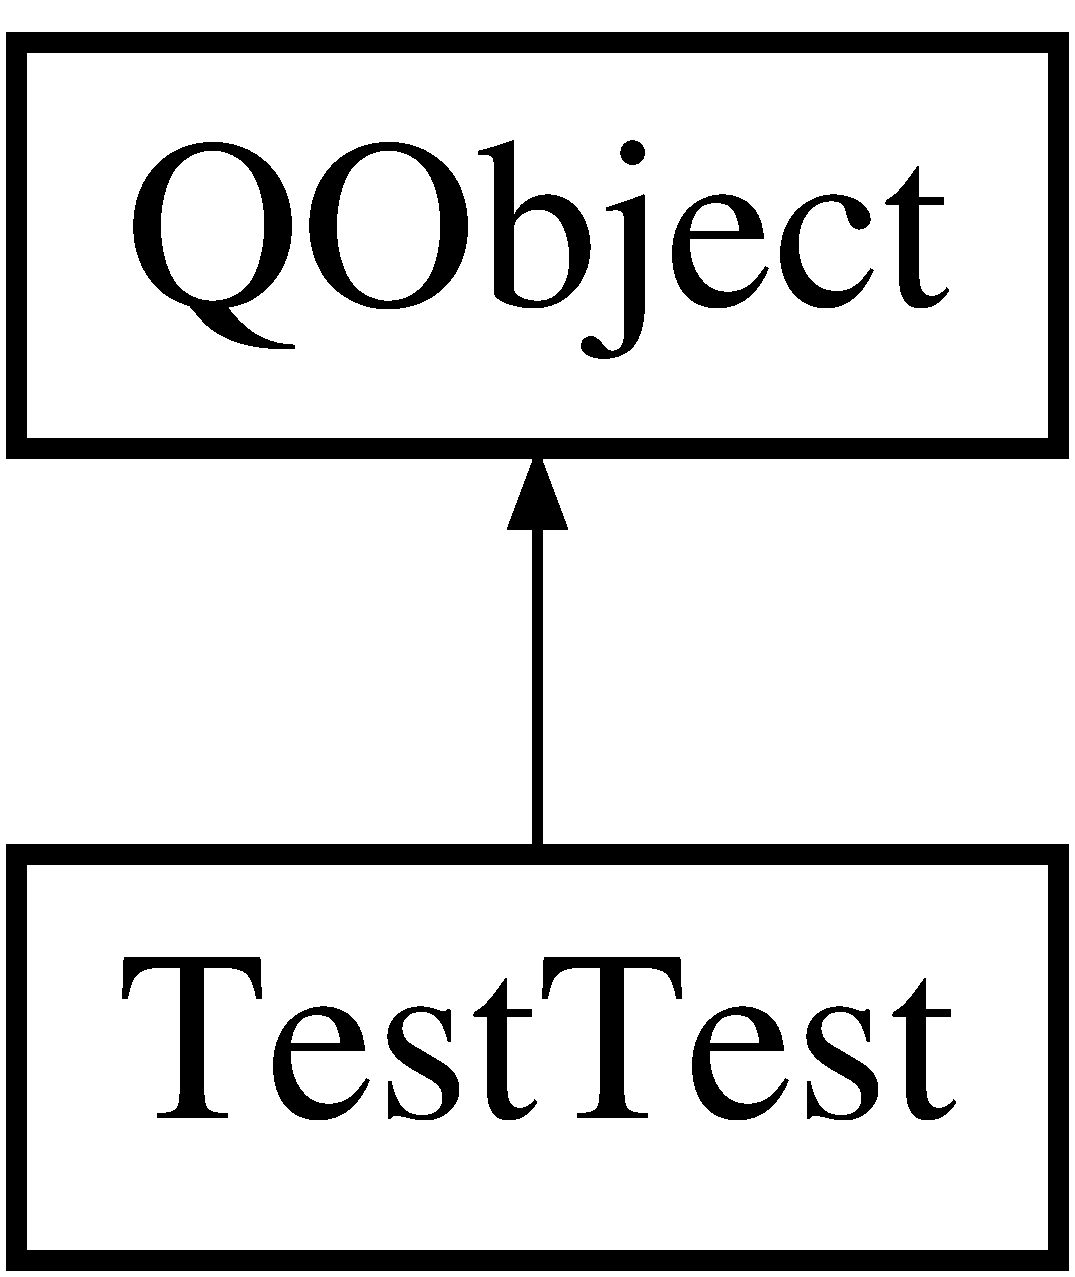
\includegraphics[height=2.000000cm]{classTestTest}
\end{center}
\end{figure}


The documentation for this class was generated from the following file\-:\begin{DoxyCompactItemize}
\item 
test/tst\-\_\-testtest.\-cpp\end{DoxyCompactItemize}

\hypertarget{classUnderNullExceptionCm}{\section{Under\-Null\-Exception\-Cm Class Reference}
\label{classUnderNullExceptionCm}\index{Under\-Null\-Exception\-Cm@{Under\-Null\-Exception\-Cm}}
}
Inheritance diagram for Under\-Null\-Exception\-Cm\-:\begin{figure}[H]
\begin{center}
\leavevmode
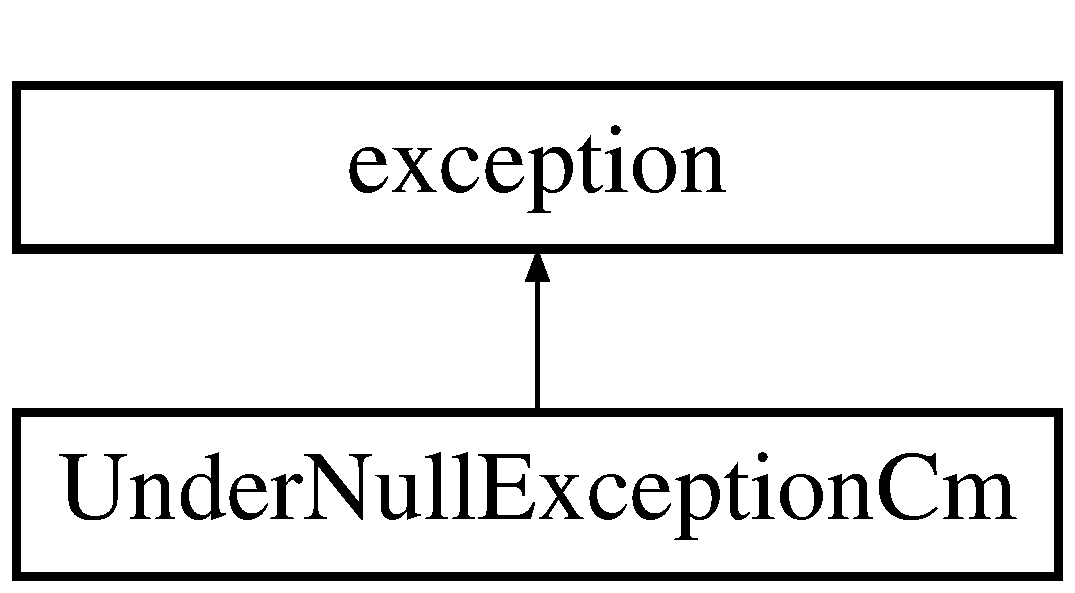
\includegraphics[height=2.000000cm]{classUnderNullExceptionCm}
\end{center}
\end{figure}
\subsection*{Public Member Functions}
\begin{DoxyCompactItemize}
\item 
\hypertarget{classUnderNullExceptionCm_a0a7dde2dc30c17111dff2fa6325f48bc}{{\bfseries Under\-Null\-Exception\-Cm} (const int cm)}\label{classUnderNullExceptionCm_a0a7dde2dc30c17111dff2fa6325f48bc}

\item 
\hypertarget{classUnderNullExceptionCm_a7a1a964ead8846f28ef1de10015c07c7}{int {\bfseries Get\-Cm} () const }\label{classUnderNullExceptionCm_a7a1a964ead8846f28ef1de10015c07c7}

\end{DoxyCompactItemize}


The documentation for this class was generated from the following file\-:\begin{DoxyCompactItemize}
\item 
lib\-C\-P\-P/exception.\-h\end{DoxyCompactItemize}

\hypertarget{classUnderNullExceptionH}{\section{Under\-Null\-Exception\-H Class Reference}
\label{classUnderNullExceptionH}\index{Under\-Null\-Exception\-H@{Under\-Null\-Exception\-H}}
}
Inheritance diagram for Under\-Null\-Exception\-H\-:\begin{figure}[H]
\begin{center}
\leavevmode
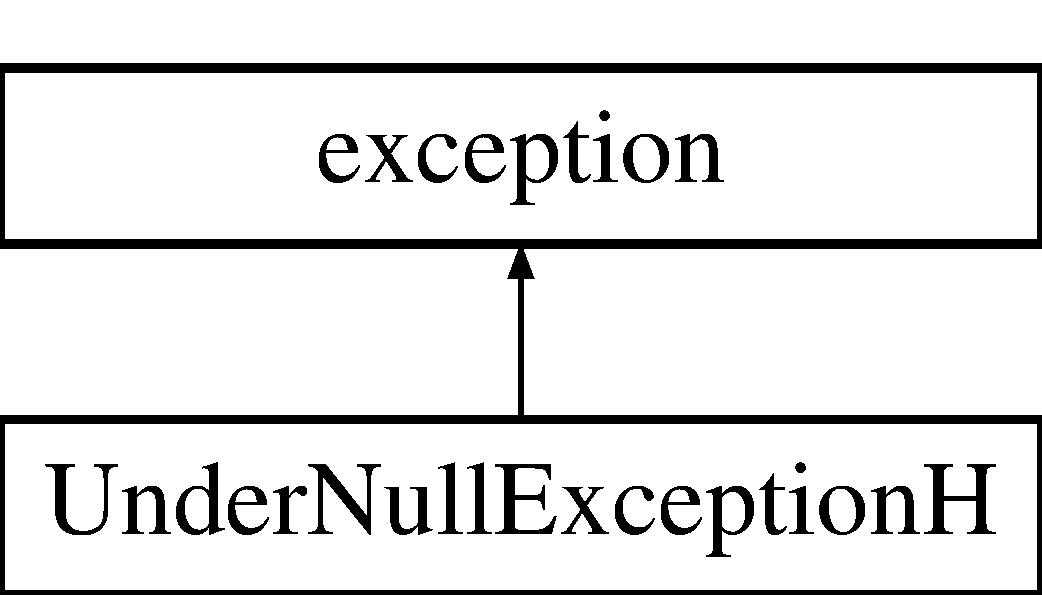
\includegraphics[height=2.000000cm]{classUnderNullExceptionH}
\end{center}
\end{figure}
\subsection*{Public Member Functions}
\begin{DoxyCompactItemize}
\item 
\hypertarget{classUnderNullExceptionH_ab3261fa1162c78661e6e466da1f278be}{{\bfseries Under\-Null\-Exception\-H} (const int height)}\label{classUnderNullExceptionH_ab3261fa1162c78661e6e466da1f278be}

\item 
\hypertarget{classUnderNullExceptionH_a4902796ebe39498e25d27accc2e85a15}{int {\bfseries Get\-Height} () const }\label{classUnderNullExceptionH_a4902796ebe39498e25d27accc2e85a15}

\end{DoxyCompactItemize}


The documentation for this class was generated from the following file\-:\begin{DoxyCompactItemize}
\item 
lib\-C\-P\-P/exception.\-h\end{DoxyCompactItemize}

\hypertarget{classUnderNullExceptionSumma}{\section{Under\-Null\-Exception\-Summa Class Reference}
\label{classUnderNullExceptionSumma}\index{Under\-Null\-Exception\-Summa@{Under\-Null\-Exception\-Summa}}
}
Inheritance diagram for Under\-Null\-Exception\-Summa\-:\begin{figure}[H]
\begin{center}
\leavevmode
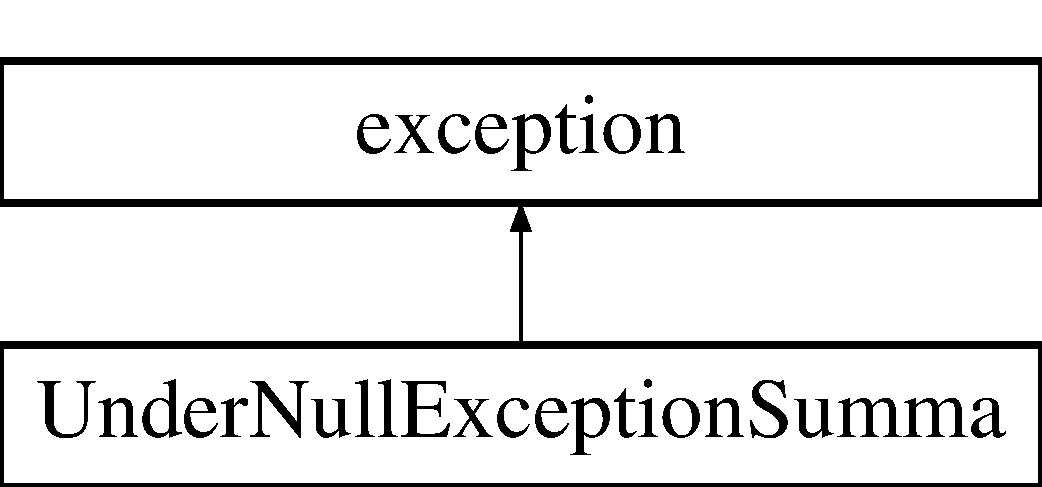
\includegraphics[height=2.000000cm]{classUnderNullExceptionSumma}
\end{center}
\end{figure}
\subsection*{Public Member Functions}
\begin{DoxyCompactItemize}
\item 
\hypertarget{classUnderNullExceptionSumma_aa2ea9ddcdbf46e8c27186a4aa3363d7d}{{\bfseries Under\-Null\-Exception\-Summa} (const int summa)}\label{classUnderNullExceptionSumma_aa2ea9ddcdbf46e8c27186a4aa3363d7d}

\item 
\hypertarget{classUnderNullExceptionSumma_a09ba48ecd331f9762d3e65898c721c2f}{int {\bfseries Get\-Summa} () const }\label{classUnderNullExceptionSumma_a09ba48ecd331f9762d3e65898c721c2f}

\end{DoxyCompactItemize}


The documentation for this class was generated from the following file\-:\begin{DoxyCompactItemize}
\item 
lib\-C\-P\-P/exception.\-h\end{DoxyCompactItemize}

\hypertarget{classUnderNullExceptionW}{\section{Under\-Null\-Exception\-W Class Reference}
\label{classUnderNullExceptionW}\index{Under\-Null\-Exception\-W@{Under\-Null\-Exception\-W}}
}
Inheritance diagram for Under\-Null\-Exception\-W\-:\begin{figure}[H]
\begin{center}
\leavevmode
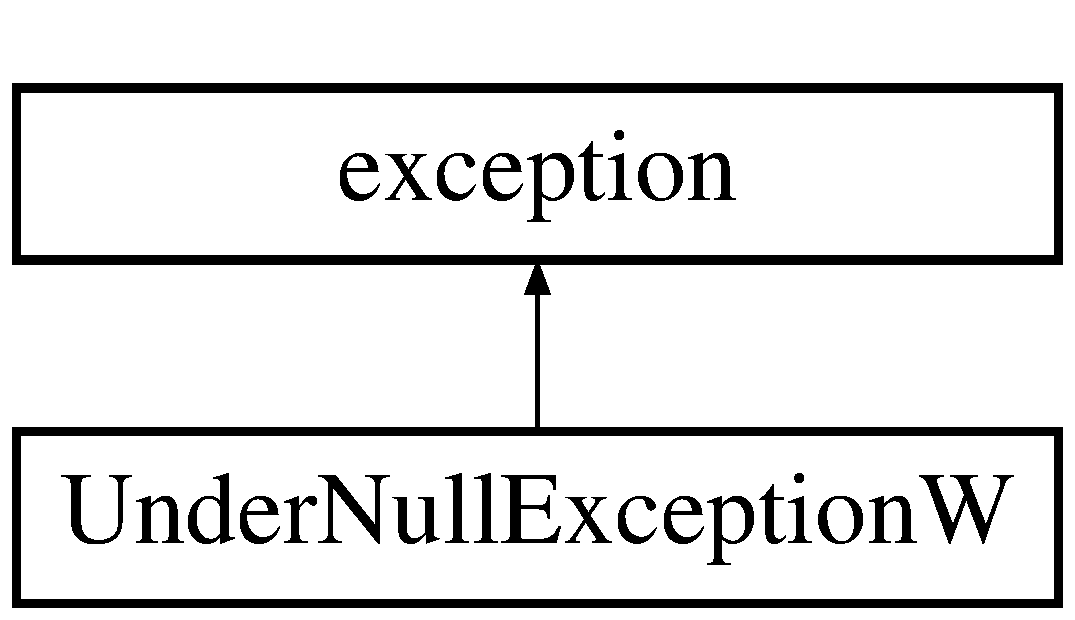
\includegraphics[height=2.000000cm]{classUnderNullExceptionW}
\end{center}
\end{figure}
\subsection*{Public Member Functions}
\begin{DoxyCompactItemize}
\item 
\hypertarget{classUnderNullExceptionW_ae4b45aecdce50c8a4dbdba6d9a2f5140}{{\bfseries Under\-Null\-Exception\-W} (const int width)}\label{classUnderNullExceptionW_ae4b45aecdce50c8a4dbdba6d9a2f5140}

\item 
\hypertarget{classUnderNullExceptionW_acf723be6bcb5b1697367a722626c21dd}{int {\bfseries Get\-Width} () const }\label{classUnderNullExceptionW_acf723be6bcb5b1697367a722626c21dd}

\end{DoxyCompactItemize}


The documentation for this class was generated from the following file\-:\begin{DoxyCompactItemize}
\item 
lib\-C\-P\-P/exception.\-h\end{DoxyCompactItemize}

%--- End generated contents ---

% Index
\newpage
\phantomsection
\addcontentsline{toc}{chapter}{Index}
\printindex

\end{document}
